\begin{figure*}
  \begin{subfigure}[b]{0.5\textwidth}
    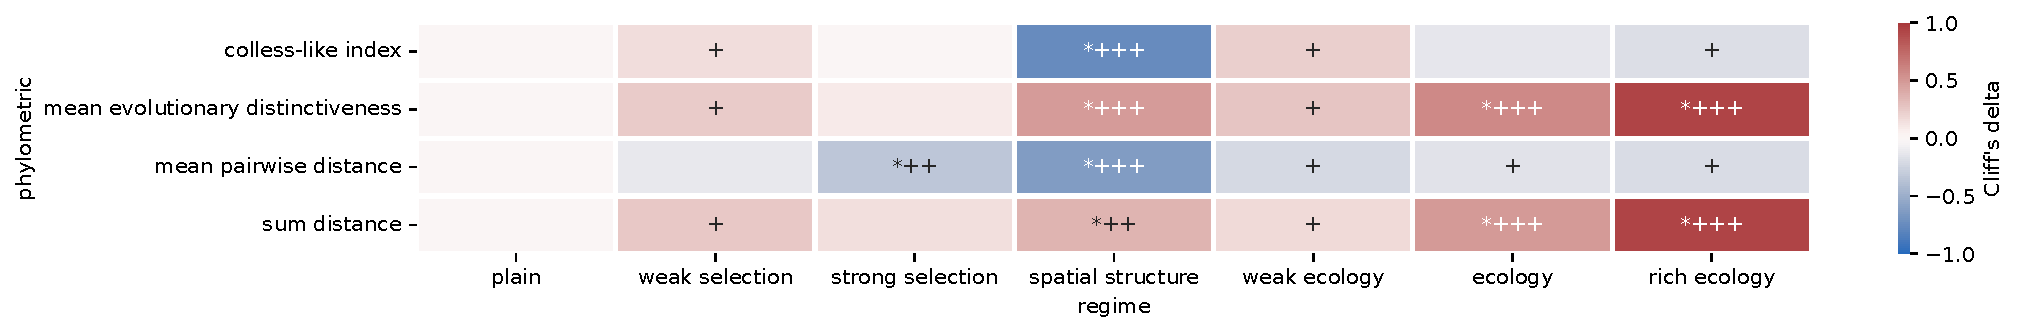
\includegraphics[width=\textwidth]{binder/binder/gen3sis/teeplots/epoch=0+mut_distn=default+viz=heatmap+x=regime+y=phylometric+ext=.pdf}
    \caption{non-spatial baseline}
    \label{fig:perfect-tree-phylometrics-heatmap-gen3sis}
  \end{subfigure}%
  \begin{subfigure}[b]{0.5\textwidth}
    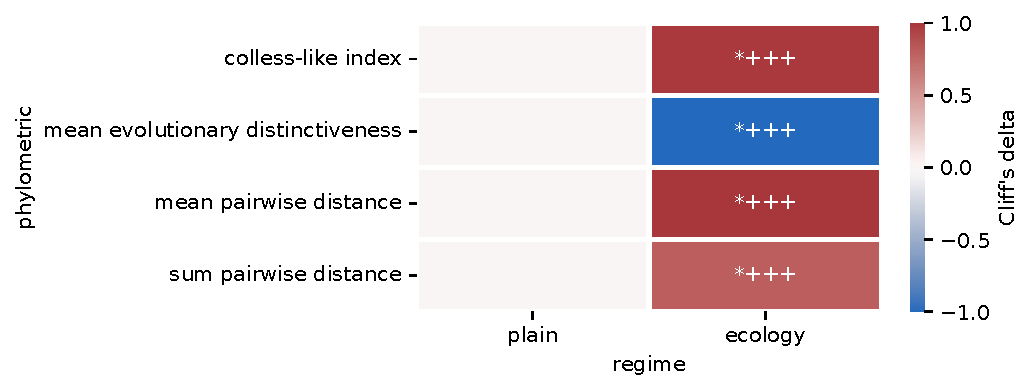
\includegraphics[width=\textwidth]{binder/binder/gen3sis/teeplots/epoch=0+mut_distn=default+spatial=true+viz=heatmap+x=regime+y=phylometric+ext=.pdf}
    \caption{spatial baseline}
    \label{fig:perfect-tree-phylometrics-spatial-heatmap-gen3sis}
  \end{subfigure}
  \caption{%
    Evolutionary regimes' effect sizes relative to ``plain'' baseline under the Gen3sis model with perfect phylogenetic tracking, normalized via Cliff's delta.
    Sample sizes $n=30$.
    Annotated +'s indicate small, medium, and large effect sizes using the Cliff's delta statistic and *'s indicate statistical significance at $\alpha = 0.05$ via Mann-Whitney U test.
  }
  \label{fig:perfect-tree-phylometrics-gen3sis}
\end{figure*}
